% compile with xelatex
% !TeX program = xelatex

%%%%%%%%%%%%%%%%%%%%%%%%%%%%%%%%%%%%%%%%%%%%%%%%%%%%%%%%%%%%%%%%%
% Compile with:
%
% $ latexmk -xelatex -pvc slides
%%%%%%%%%%%%%%%%%%%%%%%%%%%%%%%%%%%%%%%%%%%%%%%%%%%%%%%%%%%%%%%%%

%%%%%%%%%%%%%%%%%%%%%%%%%%%%%%%%%%%%%%%%%%%%%%%%%%%%%%%%%%%%%%%%%
% This document has the following requirements:
% - Fira Code
%   - see https://github.com/tonsky/FiraCode/wiki/Installing
% - Xelatex
%   - This should be automatically activated by the magic comment above,
%     But VSCode prevents this. Use the following setting to allow the
%     magic comment to work:
%     latex-workshop.latex.build.forceRecipeUsage: false
%     This setting should already be set by the workspace settings
%
% The manual is here:
% https://mirrors.dotsrc.org/ctan/macros/latex/contrib/beamer-contrib/themes/metropolis/doc/metropolistheme.pdf
%
%%%%%%%%%%%%%%%%%%%%%%%%%%%%%%%%%%%%%%%%%%%%%%%%%%%%%%%%%%%%%%%%%

%%%%%%%%%%%%%%%%%%%%%%%%%%%%%%%%%%%%%%%%%%%%%%%%%%%%%%%%%%%%%%%%%
% Trouble shotting:
%
% If you get this error:
%
%   Couldn't open `Fira Mono .cfg'
%   Sorry, but miktex-maketfm did not succeed.
%
% then go to: https://github.com/mozilla/Fira
% and download the repository, and
% install the fonts in the OTF folder.
%
%%%%%%%%%%%%%%%%%%%%%%%%%%%%%%%%%%%%%%%%%%%%%%%%%%%%%%%%%%%%%%%%%
\documentclass[aspectratio=169]{beamer}
\usepackage{amsfonts}
\usepackage{amsmath}
\usepackage{amssymb}
\usepackage{amsthm}
\usepackage{datetime}
\usepackage{flix}
\usepackage{fontspec}
\usepackage{graphicx}
\usepackage{listings}
\usepackage{lstfiracode}
\usepackage{microtype}
\usepackage{multicol}
\usepackage{oubraces}
\usepackage{pgf}
\usepackage{tikz}
\usepackage{xcolor}

\newcommand{\DayOne}{Tuesday}
\newcommand{\DayTwo}{Thursday}

\newcommand{\Highlight}[1]{\colorbox{black!10}{$\displaystyle#1$}}

\newcommand{\remark}[1]{{\color{red} \textbf{$\triangleright$ #1 $\triangleleft$}}}

\let\Code\lstinline

\lstset{language=flix}


\usetheme{metropolis}


\title{Week 1}
\date{\today{} at \currenttime{}}
\author{Magnus Madsen}

\begin{document}

\maketitle

\begin{frame}{Week 1: Outline}
\begin{columns}
\begin{column}{.05\textwidth}
\rotatebox{90}{\large \textbf{\DayOne{}}}
\end{column}
\begin{column}{.95\textwidth}
    \footnotesize
\textbf{Lecture} (45min)  \vspace{-2mm}
\begin{itemize}
    \setlength\itemsep{-0.5em}
    \item Introduction to Declarative Logic Programming
    \item Introduction to Datalog
    \item Getting Started with Datalog in Flix
\end{itemize}
\textbf{Exercises} (45min) \vspace{-2mm}
\begin{itemize}
    \item Work on the assignment alone or together in small groups.
\end{itemize}
\end{column}
\end{columns}

\medskip
\medskip
\medskip

\color{gray}
\begin{columns}
\begin{column}{.05\textwidth}
\rotatebox{90}{\large \textbf{\DayTwo{}}}
\end{column}
\begin{column}{.95\textwidth}
\footnotesize
\textbf{Lecture} (45min) \vspace{-2mm}
\begin{itemize}
    \color{gray}
    \setlength\itemsep{-0.5em}
    \item Model-Theoretic Semantics
    \item Fixpoint Semantics
    \item Stratified Negation
\end{itemize}
\textbf{Exercises} (45min)  \vspace{-2mm}
\begin{itemize}
    \color{gray}
    \item Work on the assignment alone or together in small groups.
\end{itemize}
\end{column}
\end{columns}
\end{frame}

\begin{frame}{Quote of the Day}
``To know a second language, is to have a second soul.''

\begin{flushright}
--- Charlemagne
\end{flushright}
\end{frame}

\begin{frame}{Pull Requests are Welcome}
\begin{columns}
\begin{column}{.50\textwidth}
You can improve the course material!

\begin{itemize}
    \item Exercises are in \texttt{src/weekX.md}
    \item Slides are in \texttt{slides/weekX.tex}
\end{itemize}

\medskip

PRs can be submitted on GitHub:
\begin{center}
\scriptsize
\url{https://github.com/magnus-madsen/advprog/}
\end{center}
\end{column}
\begin{column}{.50\textwidth}
    % Source: https://www.q-files.com/history/ancient-egypt/pyramids-how-they-were-built
    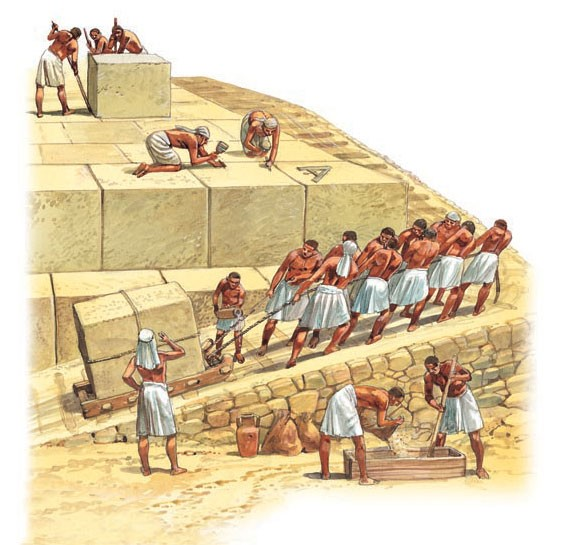
\includegraphics[width=\textwidth]{img/pyramids.jpg}
\end{column}
\end{columns}
\end{frame}


\section{Introduction to \\ Declarative Logic Programming}

\begin{frame}{Programming Paradigms}
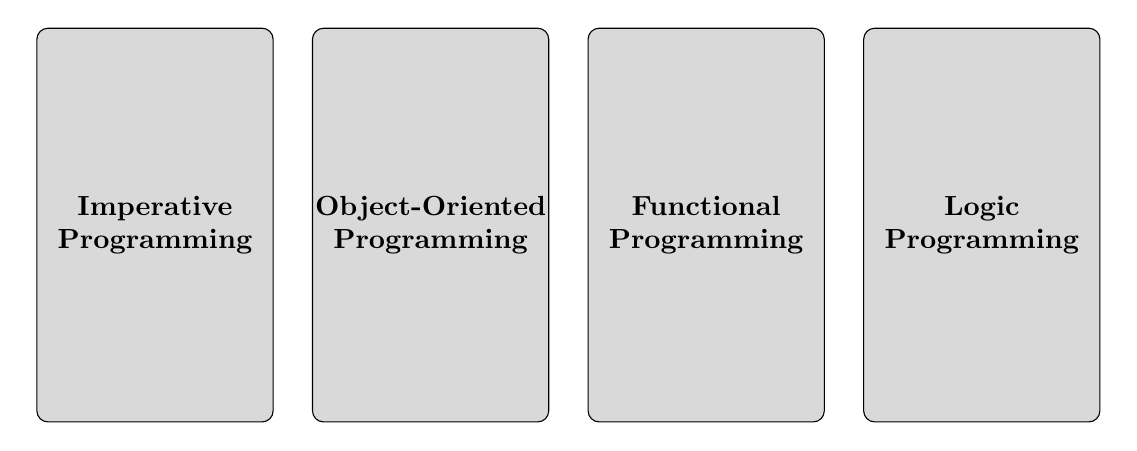
\begin{tikzpicture}
  \draw[rounded corners, fill=gray!30] (0,0) rectangle (3,5);
  \node[align=center, text width=3cm] at (1.5,2.5) {\bfseries Imperative\\Programming};

  \draw[rounded corners, fill=gray!30] (3.5,0) rectangle (6.5,5);
  \node[align=center, text width=3cm] at (5,2.5) {\bfseries Object-Oriented\\Programming};

  \draw[rounded corners, fill=gray!30] (7,0) rectangle (10,5);
  \node[align=center, text width=3cm] at (8.5,2.5) {\bfseries Functional\\Programming};

  \draw[rounded corners, fill=gray!30]  (10.5,0) rectangle (13.5,5);
  \node[align=center, text width=3cm] at (12,2.5) {\bfseries Logic\\Programming};
\end{tikzpicture}
\end{frame}

\begin{frame}{Declarative Programming}
What is a \textbf{declarative} programming language?

\bigskip

\begin{quote}
``Denoting high-level programming languages which can be used to solve problems
without requiring the programmer to specify an exact procedure to be followed.''
\begin{flushright}
--- The Oxford Dictionary
\end{flushright}
\end{quote}

\bigskip
\bigskip

\pause

\begin{quote}
\centering
\LARGE ``The \textbf{\emph{what}}, not the \textbf{\emph{how}}.''
\end{quote}
\end{frame}

\begin{frame}{Declarative Programming Languages}
Examples:

\begin{itemize}
    \item Hypertext Markup Language (HTML)
    \item Cascading Style Sheets (CSS)
    \item Structured Query Language (SQL)
    \item Regular Expressions
\end{itemize}
\end{frame}

\begin{frame}{Example: Regular Expressions}
A \textbf{\emph{regular expression}} is a declarative description of a set of strings.

For example, the regular expression $r$: 
%
$$
r = (ab)^\star + c
$$

Describes the set of strings consisting of any number of ab's or a single c.

\pause

We may want to ask: Is the string ``aba'' in the language of $r$?

We can compute the answer to this question in multiple ways:

\begin{itemize}
    \item We can construct a finite state automaton (FA) and run the string on it.
    \item We can write a regular expression interpreter and run the string on it.
\end{itemize}
\end{frame}

\begin{frame}{Why does it matter?}
In high-school you may have seen complex equations of the form:
\[
    2x = 6
\]
We can compute the solution to such an equation by various means.

\pause

\begin{itemize}
    \item Guess! (Yes, why not?) 
    \pause \item Use algebraic simplifications (subtract $x$ on both sides, and so on).
    \pause \item Rewrite the equation to a system of linear equalities and use
    Gauss-Jordan Elimination (reduction to row echelon form).
    \pause \item Rewrite the equation to a system of linear inequalities and use
    Fourier--Motzkin Elimination.
\end{itemize}

\pause

\textbf{Upshot}: We agree on the meaning of the equation and we can \emph{check}
whether a proposed solution is a \emph{valid} solution.
\end{frame}

\begin{frame}{Logic Programming}
What is a \textbf{logic} programming language?

\bigskip

\begin{quote}
``Logic programming is a type of programming paradigm which is largely based on
formal logic. Any program written in a logic programming language is a set of
sentences in logical form, expressing facts and rules about some problem
domain.''
\begin{flushright}
--- Wikipedia
\end{flushright}
\end{quote}
\end{frame}

\begin{frame}{Declarative Logic Programming}
The programmer writes a collection of \textbf{logic constraints}.

\pause

The compiler and runtime \textbf{computes the solution} to the constraints.

\begin{itemize}
    \item It freely chooses the algorithms and data structures required to do so.
    \begin{itemize}
        \item For example, it might solve the constraints in parallel.
    \end{itemize}
\end{itemize}

\pause

Declarative logic programming offers several benefits:

\begin{itemize}
    \pause \item no side-effects + no explicit control-flow
    \begin{itemize}
        \item Programs are easy to understand.
        \item Programs are easy to modify and extend.
        \item Programs can be structured in any order.
    \end{itemize}
    \pause \item Strong guarantees about termination.
\end{itemize}

\pause

\textbf{Challenge}: Logic programming requires a different mindset.
\end{frame}

\section{Introduction to Datalog}

\begin{frame}{Datalog}
\textbf{Datalog} is a simple, yet powerful declarative logic programming language.
\begin{itemize}
    \pause \item Research on Datalog goes back to the 1970s in the fields of artificial
    intelligence, deductive databases, and knowledge representation.
    \pause \item Datalog (and Prolog) are cornerstones of classical A.I. based on
    symbolic reasoning --- before the golden age of machine learning.
\end{itemize}

\pause

A Datalog program is essentially a collection of \emph{Horn clauses}:
%
$$
\forall x_1, \cdots, x_n. \, P_0(t \cdots) \Leftarrow P_1(t \cdots), \cdots, P_m(t \cdots).
$$
which allow us to derive new knowledge from existing knowledge.

\pause

Datalog and Prolog are closely related, but should not be confused.
\end{frame}

\begin{frame}{Real-World Applications}
Datalog has been successfully used in a range of applications:

\begin{itemize}
    \item in large-scale points-to analysis of Java programs.
    \item as an alternative foundation for the Rust borrow checker.
    \item to identify misconfigurations or security vulnerabilities in AWS networks.
\end{itemize}

\pause

Datalog is a surgical instrument: You use it when the problem calls for it. 
\end{frame}

\begin{frame}{Expressive Power}
\centering
\medskip
\medskip
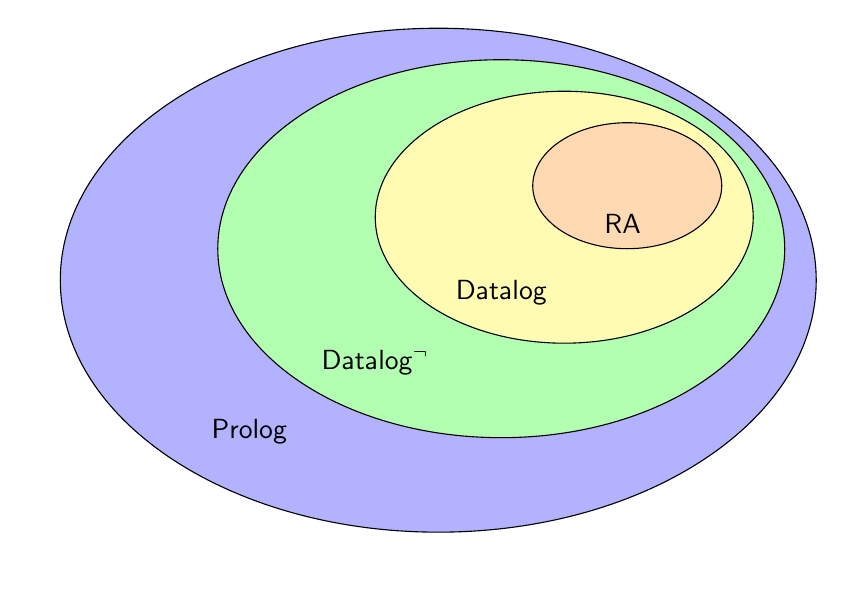
\begin{tikzpicture}[font=\sffamily, scale=0.8]
\foreach \X/\col [count=\N, evaluate=\N as \Y using 5-\N] in {Prolog/blue, Datalog$^\neg$/green, Datalog/yellow, RA /orange}
{\draw[fill=\col!30] (-\Y,-\Y/2) circle ({1.5*\Y} and \Y);
\node[align=center] at (1-2*\Y,-1.1*\Y) {\X}; }
\draw ([xshift=-0.5cm,yshift=-0.5cm] current bounding box.south west);
\end{tikzpicture}
\end{frame}

\begin{frame}[fragile]{Example}
Find a \textbf{one-way} trip from Toronto to Billund with the same airline.

\begin{lstlisting}[language=flix, xleftmargin=0.8cm]
Route(x, airline, y) :- Leg(x, airline, y).
Route(x, airline, z) :- 
    Route(x, airline, y),
    Leg(y, airline, z).

OneWay(airline) :- Route("YYZ", airline, "BLL").
\end{lstlisting}

\pause

Find a \textbf{round-trip} from Toronto to Billund with the same airline.

\begin{lstlisting}[language=flix, xleftmargin=0.8cm]
TwoWay(airline) :- 
    Route("YYZ", airline, "BLL"), 
    Route("BLL", airline, "YYZ").
\end{lstlisting}
\end{frame}

\begin{frame}{Datalog Programs}
A Datalog \textbf{program} $p$ is a finite sequence of constraints:
%
{\Large
\begin{align*}
p \in \textsl{Program} = c_1 \cdots c_n
\end{align*}
}

\pause

The order of constraints is immaterial.

\pause

Note: The shortest Datalog program is the empty sequence of constraints.
\end{frame}

\begin{frame}{Datalog Constraints}
A Datalog \textbf{constraint} $c$ consists of a \textbf{head} and a \textbf{body}:
%
{\Large
\begin{align*}
c \in \textsl{Constraint} = A_0 \Leftarrow A_1, \cdots, A_n.
\end{align*}
}

\pause

Each $A_i$ is an atom. The atom $A_0$ is the head. The atoms $A_1, \cdots, A_N$ are the body. 

\pause

The sequence of body atoms may be empty.

\pause

A \textbf{fact} is a constraint with an empty body.

A \textbf{rule} is a constraint with a non-empty body.
\end{frame}

\begin{frame}{Datalog Atoms and Terms}

A Datalog atom $A$ is a predicate symbol and a finite sequence of terms:
%
{\Large
\begin{align*}
A \in \textsl{Atom} = p(t_1, \cdots, t_n)
\end{align*}
}

A predicate symbol $p$ is an identifier, i.e. a name. 

\pause

A term $t$ is either a constant $k$ or a variable $x$:
%
{\Large
\begin{align*}
t \in \textsl{Term} = k \mid x.
\end{align*}
}

A constant $k$ is a primitive value, e.g. a number of string.
\end{frame}

\begin{frame}[fragile]{Datalog Grammar}
The complete grammar for Datalog is:
%
{
\large
\begin{align*}
p \in \textsl{Program}      &= c_1 \cdots c_n \\
c \in \textsl{Constraint}   &= A_0 \Leftarrow A_1, \cdots, A_n. \\ 
A \in \textsl{Atom}         &= p(t_1, \cdots, t_n) \\
t \in \textsl{Term}         &= k \mid x. \\
\\
p \in \textsl{Predicates}   & = \text{is a finite set of predicate symbols.} \\
x \in \textsl{Variables}    & = \text{is a finite set of variable symbols.} \\
k \in \textsl{Constants}    & = \text{is a finite set of constants.}
\end{align*}
}
\end{frame}

\begin{frame}{Example}
\Large
\begin{equation*}
\overunderbraces{&\br{3}{\text{\bfseries Rule}}}%
{&\textsf{OneWay}(\textsf{airline}) & \Leftarrow & \textsf{Route}(\textsf{"YYZ"}, \textsf{airline}, \textsf{"BLL"}).&}%
{&\br{1}{\text{\bfseries Head}} & & \br{1}{\text{\bfseries Body}}}
\end{equation*}

\begin{equation*}
\overunderbraces{&\br{8}{\text{\bfseries Atom}}}%
{&\textsf{Route} & (&\textsf{"YYZ"}&, &\textsf{airline}&, &\textsf{"BLL"}&).&}%
{&\br{2}{\text{\bfseries Predicate}} &\br{1}{\text{\bfseries Const}} & &\br{1}{\text{\bfseries Var}} & &\br{1}{\text{\bfseries Const}} }
\end{equation*}
\end{frame}

\begin{frame}[fragile]{Ground Atoms and Rules}
An \textbf{atom} is said to be \textbf{ground} if it does not contain a variable.

A \textbf{rule} is said to be \textbf{ground} if it all of its atoms are ground.

For example:
\begin{lstlisting}[language=flix,xleftmargin=0.8cm]
A(1, 2, 3).                // Ground Atom
A(1, 2, 3) :- B(2), C(3).  // Ground Rule
\end{lstlisting}
\end{frame}

\begin{frame}[fragile]{Safety}
A Datalog program $P$ is \textbf{safe} if:
\begin{enumerate}
    \item Every fact in $P$ is ground.
    \item Every variable $x$ that occurs in the head of a rule also occurs in
    its body\footnote{This is sometimes called the \textsl{range restriction
    property}.}.
\end{enumerate}

For example:
\begin{lstlisting}[language=flix,xleftmargin=0.8cm]
A(1, x).             // unsafe, violates (1)
A(x, y) :- B(x).     // unsafe, violates (2)
A(x, _) :- B(x).     // unsafe, violates (2)
A(1, x) :- C(x, y).  // OK
\end{lstlisting}
\end{frame}

\begin{frame}{Theoretical Properties}
Datalog has several important theoretical properties:

\begin{itemize}
    \item Every Datalog program has a unique solution.
    \item Every Datalog program eventually terminates.
    \item Every polynomial time algorithm can be expressed in Datalog.
\end{itemize}

\medskip

\pause

\textbf{Upshot}: Debugging is easy! 

\end{frame}

\begin{frame}[fragile]{A Larger Example (1/2)}
\begin{columns}
\begin{column}{.65\textwidth}
\begin{lstlisting}[language=flix]
Friend("Cartman", "Kyle").
Friend("Cartman", "Stan").
Friend("Kyle", "Cartman").
Friend("Kyle", "Stan").
Friend("Stan", "Cartman").
Friend("Stan", "Kyle").
Friend("Stan", "Wendy").
Friend("Wendy", "Stan").


Interest("Cartman", "Politics").
Interest("Cartman", "Guitar Hero").
Interest("Kyle", "Guitar Hero").
Interest("Stan", "Guitar Hero").
Interest("Wendy", "Politics").
\end{lstlisting}
\end{column}
\begin{column}{.35\textwidth}
\begin{center}

\includegraphics[width=0.9\textwidth]{img/southpark.jpg}
\end{center}
\end{column}
\end{columns}
\end{frame}

\begin{frame}[fragile]{A Larger Example (2/2)}
\begin{columns}
\begin{column}{.5\textwidth}
\begin{lstlisting}[language=flix]
Friend("Cartman", "Kyle").
Friend("Cartman", "Stan").
Friend("Kyle", "Cartman").
Friend("Kyle", "Stan").
Friend("Stan", "Cartman").
Friend("Stan", "Kyle").
Friend("Stan", "Wendy").
Friend("Wendy", "Stan").


Interest("Cartman", "Politics").
Interest("Cartman", "Guitar Hero").
Interest("Kyle", "Guitar Hero").
Interest("Stan", "Guitar Hero").
Interest("Wendy", "Politics").
\end{lstlisting}
\end{column}
\begin{column}{.5\textwidth}
\begin{lstlisting}[language=flix]
FriendOfFriend(x, z) :- 
    Friend(x, y), 
    Friend(y, x), 
    Friend(y, z), 
    if x != z.

ShareInterest(x, y) :- 
    Interest(x, i), 
    Interest(y, i), 
    if x != y.

FriendSuggestion(x, y) :- 
    FriendOfFriend(x, y), 
    ShareInterest(x, y), 
    not Friend(x, y).
\end{lstlisting}
\end{column}
\end{columns}
\end{frame}

\section{Getting Started with Datalog in Flix}

\begin{frame}{Theory vs. Practice}
We study Datalog in its purest form: as a minimal calculus.
\begin{itemize}
    \item A bit like the lambda calculus of logic programming. 
    \item In real life, no one writes functional programs in the pure lambda calculus. 
    \item Similarly, no one writes logic programs in pure Datalog.
\end{itemize}

\pause

In practice, we want a \emph{programming language} with amenities like:
\begin{itemize}
    \item extensions that increase the expressive power.
    \item type systems to prevent mistakes.
    \item IDE support.
    \item ... and more ...
\end{itemize}
\end{frame}

\begin{frame}{Datalog Dialects and Implementations (1/2)}
There are many object-oriented languages:
\begin{itemize}
    \item E.g. Java, C\#, JavaScript, Python, Smalltalk, ...
\end{itemize}

\pause

There are many relational database management systems:
\begin{itemize}
    \item E.g. MSSQL, MySQL, Oracle DBMS, IBM DB2, SQLite, ...
\end{itemize}

\pause

In the same vein, there are also many Datalog dialects and solvers:

\begin{itemize}
    \item DLV is an established commercial Datalog engine {\small
    \url{https://www.dlvsystem.it/}}
    \item Logica is an open source Datalog engine released by Google
    \small
    \url{https://logica.dev/}
    \item Souffle is a open source and highly scalable Datalog engine {\small
    \url{https://souffle-lang.github.io/}}
\end{itemize}
\end{frame}

\begin{frame}{Datalog Dialects and Implementations (2/2)}
In this course, we shall use the \textbf{Flix programming language}:
\begin{itemize}
    \item Flix is fully-blown functional, logic, and imperative programming
    language. 
    \item A unique feature of Flix is its support for Datalog as a
    strongly-typed deeply embedded domain specific language (EDSL).
    \item Flix is developed by researchers from several universities, including
    Aarhus University, the University of Waterloo (Canada), the University of
    Copenhagen, and the University of Tubingen (Germany).
\end{itemize}  
\end{frame}

\begin{frame}{The Flix Playground (1/2)}
Flix has an online playground available at:

\bigskip
\bigskip

\begin{center}
\LARGE
\url{https://play.flix.dev/}
\end{center}

\bigskip
\bigskip

Note: The playground runs on a shared server and may be slow.

\end{frame}

\begin{frame}{The Flix Playground (2/2)}
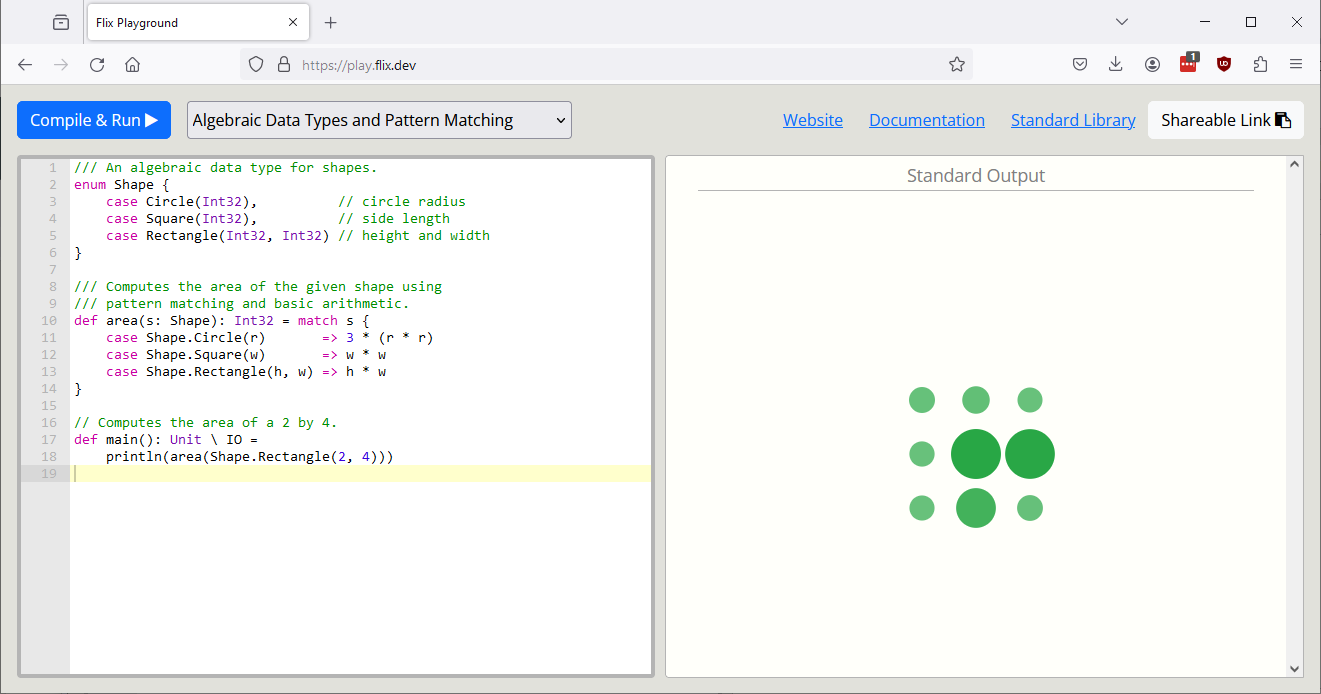
\includegraphics[width=\textwidth]{img/flix-playground.png}
\end{frame}

\begin{frame}{The Flix VSCode Extension (1/2)}
Flix has a fully-featured Visual Studio Code (VSCode) extension. 

To run Flix on your machine:
\begin{itemize}
    \item Ensure that you have Visual Studio Code installed.
    \item Ensure that you have Java 21 (or later) installed.
    \begin{itemize}
        \item \url{https://adoptium.net/}
    \end{itemize}
    \item Follow the instructions at:
    \begin{itemize}
        \item \url{https://flix.dev/get-started/}
    \end{itemize}
\end{itemize}

{\small Note: VSCode must be used in project mode, i.e. ``File -> Open Folder''.}
\end{frame}

\begin{frame}{The Flix VSCode Extension (2/2)}
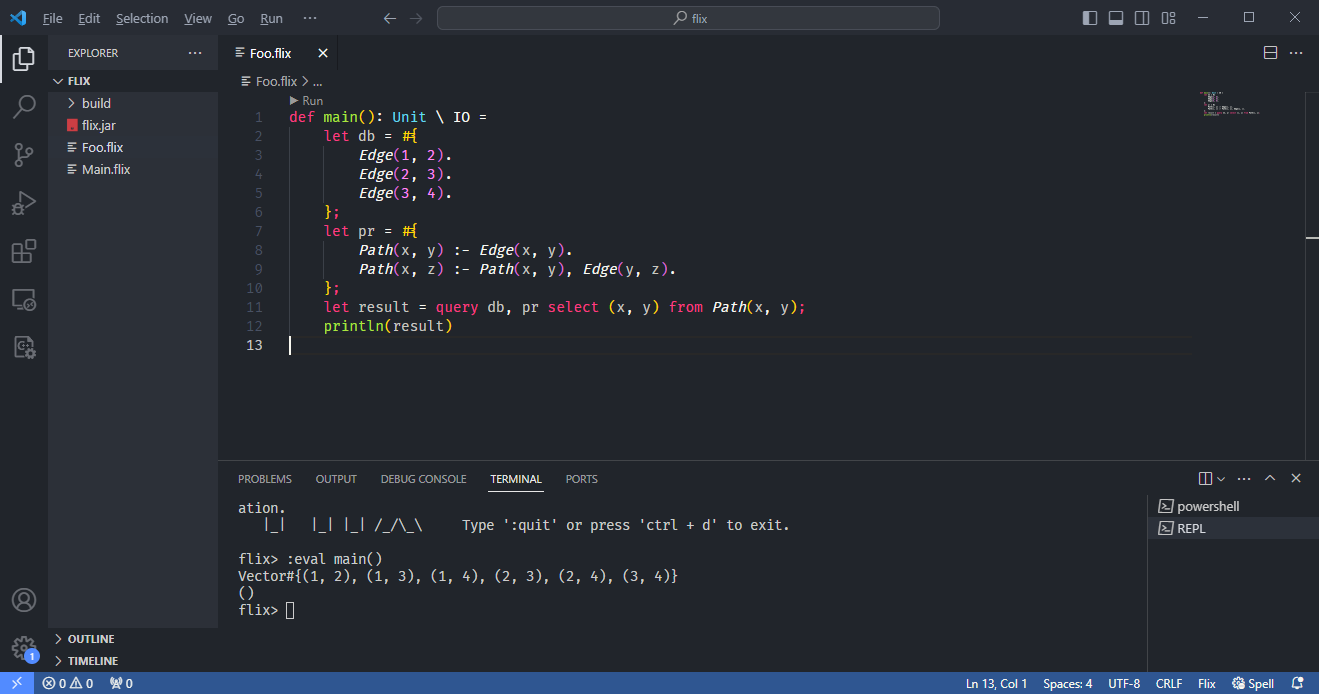
\includegraphics[width=\textwidth]{img/flix-vscode.png}
\end{frame}
    
\begin{frame}[fragile]{Flix -- An Example to Get You Started}
Here is a simple example program you can copy-and-paste to get started:
\begin{lstlisting}[language=flix]
def main(): Unit \ IO = 
    let db = #{
        Edge(1, 2).
        Edge(2, 3).
        Edge(3, 4).
    };
    let pr = #{
        Path(x, y) :- Edge(x, y).
        Path(x, z) :- Path(x, y), Edge(y, z).
    };
    let result = query db, pr select (x, y) from Path(x, y);
    println(result)
\end{lstlisting}
\end{frame}

\begin{frame}{Summary}
Declarative Programming
\begin{itemize}
    \item the \textbf{\emph{what}}, not the \textbf{\emph{how}}.
\end{itemize}

\pause

Logic programming
\begin{itemize}
    \item programs as logic constraints: \textbf{\emph{facts}} and \textbf{\emph{rules}}.
    \item infer new knowledge from existing knowledge.
\end{itemize}

\pause

\textbf{Datalog} is a simple, yet powerful \emph{declarative} \emph{logic}
programming language.
\begin{itemize}
    \item a Datalog program is a collection of facts and rules. 
    \item every Datalog program has a unique and efficiently computable solution.
\end{itemize}
\end{frame}

\begin{frame}[standout]
% blank
\end{frame}

\begin{frame}{Week 1: Outline}

\color{gray}
\begin{columns}
\begin{column}{.05\textwidth}
\rotatebox{90}{\large \textbf{\DayOne{}}}
\end{column}
\begin{column}{.95\textwidth}
    \footnotesize
\textbf{Lecture} (45min)  \vspace{-2mm}
\begin{itemize}
    \color{gray}
    \setlength\itemsep{-0.5em}
    \item Introduction to Declarative Logic Programming
    \item Introduction to Datalog
    \item Getting Started with Datalog in Flix
\end{itemize}
\textbf{Exercises} (45min) \vspace{-2mm}
\begin{itemize}
    \color{gray}
    \item Work on the assignment alone or together in small groups.
\end{itemize}
\end{column}
\end{columns}

\medskip
\medskip
\medskip

\color{black}
\begin{columns}
\begin{column}{.05\textwidth}
\rotatebox{90}{\large \textbf{\DayTwo{}}}
\end{column}
\begin{column}{.95\textwidth}
\footnotesize
\textbf{Lecture} (45min) \vspace{-2mm}
\begin{itemize}
    \setlength\itemsep{-0.5em}
    \item Model-Theoretic Semantics
    \item Fixpoint Semantics
    \item Stratified Negation
\end{itemize}
\textbf{Exercises} (45min)  \vspace{-2mm}
\begin{itemize}
    \item Work on the assignment alone or together in small groups.
\end{itemize}
\end{column}
\end{columns}
\end{frame}

\begin{frame}{Quote of the Day}
``A language that doesn't affect the way you think about programming, is not
worth knowing.''

\begin{flushright}
--- Alan Perlis
\end{flushright}
\end{frame}

\begin{frame}{Pull Requests are Welcome}
\begin{columns}
\begin{column}{.50\textwidth}
You can improve the course material!

\begin{itemize}
    \item Exercises are in \texttt{src/weekX.md}
    \item Slides are in \texttt{slides/weekX.tex}
\end{itemize}

\medskip

PRs can be submitted on GitHub:
\begin{center}
\scriptsize
\url{https://github.com/magnus-madsen/advprog/}
\end{center}
\end{column}
\begin{column}{.50\textwidth}
    % Source: https://www.q-files.com/history/ancient-egypt/pyramids-how-they-were-built
    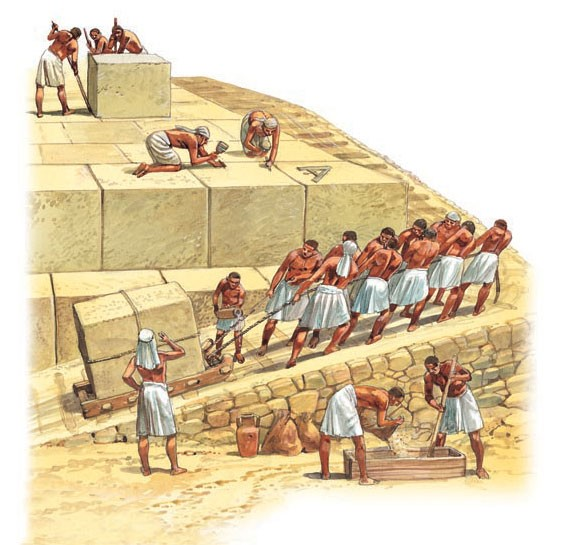
\includegraphics[width=\textwidth]{img/pyramids.jpg}
\end{column}
\end{columns}
\end{frame}


\section{Model-Theoretic Semantics}

\begin{frame}{Extensional vs. Intensional}
Given a Datalog program $P$:
\begin{itemize}
    \item The \textbf{\emph{extensional database (EDB)}} is the set of facts
    already in $P$.
    \item The \textbf{\emph{intensional database (IDB)}} is the set of facts
    derivable from $P$.
\end{itemize}

\pause

An \textbf{extensional} definition defines an object by \textbf{enumeration}.
\begin{itemize}
    \item E.g. a fruit is an apple, or an apricot, or an avocado, or a banana, or …
\end{itemize}

\pause

An \textbf{intensional} definition defines an object by its \textbf{necessary
and sufficient conditions}.
\begin{itemize}
    \item E.g. a fruit is the sweet and fleshy product of a tree or other plant that contains seed and can be eaten as food.
\end{itemize}    
\end{frame}

\begin{frame}{Model-theoretic Semantics (1/2)}
The \textbf{model-theoretic} semantics define the meaning of a Datalog program
in terms of interpretations and models. Briefly,
\begin{itemize}
    \item An interpretation is a set of facts.
    \item A model is an interpretation that satisfy all constraints in the program.
    \item The minimal model, which is unique, is smaller than all other models.
        \begin{itemize}
            \item We think of the minimal model as the solution to a Datalog program.
        \end{itemize}
\end{itemize}

\pause

The model-theoretic semantics describes the \textbf{\emph{what}}, not the
\textbf{\emph{how}}.
\end{frame}

\begin{frame}{Model-theoretic Semantics (1/2)}
We will need to learn several new definitions and concepts:
\begin{itemize}
    \item Herbrand Base and Herbrand Universe
    \item Interpretations
    \item Truth
    \item Models
    \item Minimality
\end{itemize}

But fear not, these definitions and concepts are not too difficult.
\end{frame}

\begin{frame}[fragile]{Running Example}
\begin{columns}
\begin{column}{.65\textwidth}
We will use the following simple Datalog program $P$:

\medskip

\begin{lstlisting}[language=flix]
GrandParent(x, z) :- Parent(x, y), Parent(y, z).

Parent("Bart", "Homer").
Parent("Lisa", "Homer").
Parent("Homer", "Grampa").
\end{lstlisting}
\end{column}
\begin{column}{.35\textwidth}
\begin{flushright}

\includegraphics[width=0.9\textwidth]{img/simpsons.png}
\end{flushright}
\end{column}
\end{columns}
\end{frame}

\begin{frame}{Herbrand Universe}
The \textbf{\emph{Herbrand Universe}} $\mathcal{U}$ of a Datalog program $P$ is
\textbf{the set of all constants} appearing anywhere in $P$.

For example, the Herbrand Universe of $P$ is the set:
%
\Large
$$
U = \{ \textsf{"Bart"}, \textsf{"Lisa"}, \textsf{"Homer"}, \textsf{"Grampa"} \}
$$
\end{frame}

\begin{frame}{Herbrand Base}
The Herbrand Base $\mathcal{B}$ of a Datalog program $P$ is the set of all
ground atoms with predicates symbols drawn from $P$ and terms drawn from the
Herbrand Universe $\mathcal{U}$.

For our example, the Herbrand Base of $P$ is the set:
\small
$$
B = \left\{
\begin{array}{ll}
\textsf{Parent}(\textsf{"Bart"}, \textsf{"Bart"}),      & \textsf{GrandParent}(\textsf{"Bart"}, \textsf{"Bart"}), \\
\textsf{Parent}(\textsf{"Bart"}, \textsf{"Lisa"}),      & \textsf{GrandParent}(\textsf{"Bart"}, \textsf{"Lisa"}), \\
\textsf{Parent}(\textsf{"Bart"}, \textsf{"Homer"}),     & \textsf{GrandParent}(\textsf{"Bart"}, \textsf{"Homer"}), \\
\textsf{Parent}(\textsf{"Bart"}, \textsf{"Grampa"}),    & \textsf{GrandParent}(\textsf{"Bart"}, \textsf{"Grampa"}), \\
\textsf{Parent}(\textsf{"Lisa"}, \textsf{"Bart"}),      & \textsf{GrandParent}(\textsf{"Lisa"}, \textsf{"Bart"}), \\
\textsf{Parent}(\textsf{"Lisa"}, \textsf{"Lisa"}),      & \textsf{GrandParent}(\textsf{"Lisa"}, \textsf{"Lisa"}), \\
\textsf{Parent}(\textsf{"Lisa"}, \textsf{"Homer"}),     & \textsf{GrandParent}(\textsf{"Lisa"}, \textsf{"Homer"}), \\
\textsf{Parent}(\textsf{"Lisa"}, \textsf{"Grampa"}),    & \textsf{GrandParent}(\textsf{"Lisa"}, \textsf{"Grampa"}), \\
\cdots & \cdots \\ 
\textsf{Parent}(\textsf{"Grampa"}, \textsf{"Grampa"}),  & \textsf{GrandParent}(\textsf{"Grampa"}, \textsf{"Grampa"}), \\
\end{array}\right\}
$$
\end{frame}

\begin{frame}{Interpretations}
An \textbf{interpretation} $I \subseteq \mathcal{B}$ is a subset of the Herbrand
Base.

For example,
$$
I = \left\{
\begin{array}{ll}
\textsf{Parent}(\textsf{"Bart"}, \textsf{"Homer"}),      & \textsf{GrandParent}(\textsf{"Bart"}, \textsf{"Grampa"}), \\
\textsf{Parent}(\textsf{"Lisa"}, \textsf{"Homer"}),      & \textsf{GrandParent}(\textsf{"Bart"}, \textsf{"Lisa"})
\end{array}\right\}
$$
is an interpretation.
\end{frame}

\begin{frame}{Truth w.r.t. an Interpretation}
Given an interpretation $I$ we can determine the truth of a constraint:
\begin{itemize}
    \item A ground atom $A = p(k_1, \cdots, k_n)$ is true w.r.t. an
    interpretation $I$ if $A \in I$.
    \item A conjunction of ground atoms $A_1, \cdots, A_n$ is true w.r.t. an
    interpretation $I$ if each atom $A_i$ is true in the interpretation.
    \item A ground rule $A_0 \Leftarrow A_1, \cdots, A_n$ is true w.r.t. an
    interpretation if the body conjunction $A_1, \cdots, A_n$ is false or the
    head atom $A_0$ is true.
\end{itemize}
\end{frame}

\begin{frame}{Example}
Given the interpretation:
$$
I = \left\{
\begin{array}{ll}
\textsf{Parent}(\textsf{"Bart"}, \textsf{"Homer"}),      & \textsf{GrandParent}(\textsf{"Bart"}, \textsf{"Grampa"}), \\
\textsf{Parent}(\textsf{"Lisa"}, \textsf{"Homer"}),      & \textsf{GrandParent}(\textsf{"Bart"}, \textsf{"Lisa"})
\end{array}\right\}
$$

\pause

The ground atom:
$$
\textsf{Parent}(\textsf{"Lisa"}, \textsf{"Homer"})
$$
is true.

\pause

Moreover, the ground rule:
$$
\textsf{GrandParent}(\textsf{"Lisa"}, \textsf{"Lisa"}) \Leftarrow \textsf{Parent}(\textsf{"Bart"}, \textsf{"Homer"}), \textsf{Parent}(\textsf{"Homer"}, \textsf{"Grampa"}).
$$
is true.
\end{frame}

\begin{frame}{Models}
A \textbf{model} $M$ of a Datalog program $P$ is an interpretation $I$ that
makes each ground instance of each constraint in $P$ true.

\pause

A \emph{ground instance} of a rule is obtained by replacing every variable in a
rule with a constant from the Herbrand universe. For example, the
interpretation:
$$
M = \left\{
\begin{array}{ll}
\textsf{Parent}(\textsf{"Bart"}, \textsf{"Homer"}),     & \textsf{GrandParent}(\textsf{"Bart"}, \textsf{"Grampa"}), \\
\textsf{Parent}(\textsf{"Lisa"}, \textsf{"Homer"}),     & \textsf{GrandParent}(\textsf{"Lisa"}, \textsf{"Grampa"}), \\
\textsf{Parent}(\textsf{"Homer"}, \textsf{"Grampa"})
\end{array}\right\}
$$
is a model of the program.
\end{frame}

\begin{frame}{Minimal Models (1/2)}
A model $M$ is \textbf{minimal} if there is no other model $M'$ such that $M'
\subset M$.

\pause

For example, the interpretation on the previous slide was a minimal model.

\pause

On other hand, the interpretation:
$$
M = \left\{
\begin{array}{ll}
\textsf{Parent}(\textsf{"Bart"}, \textsf{"Homer"}),     & \textsf{GrandParent}(\textsf{"Bart"}, \textsf{"Grampa"}), \\
\textsf{Parent}(\textsf{"Lisa"}, \textsf{"Homer"}),     & \textsf{GrandParent}(\textsf{"Lisa"}, \textsf{"Grampa"}), \\
\textsf{Parent}(\textsf{"Homer"}, \textsf{"Grampa"}),   & \textsf{GrandParent}(\textsf{"Homer"}, \textsf{"Homer"})
\end{array}\right\}
$$
is a \textbf{model}, but it is \textbf{not minimal}.

\pause

Intuition: A model satisfies the constraints, but may contain superfluous facts.
\end{frame}

\begin{frame}{Minimal Models (2/2)}
\textbf{Theorem}: Given two models $M_1$ and $M_2$ of a Datalog program $P$ the
intersection $M_1 \cap M_2$ is also a model of $P$. 

\textbf{Theorem}: The minimal model is the intersection of all models.

\textbf{Upshot}: The minimal model is unique!
\end{frame}

\section{Fixpoint Semantics}

\begin{frame}{Computing Minimal Models (1/4)}
We now have the mathematical foundations to answer questions such as:
\begin{itemize}
\item When is an interpretation a model?
\item When is a model minimal?
\item What is the solution to a Datalog program?
\end{itemize}

\pause

What we \emph{lack} is method to \textbf{compute} the minimal model of a program.
\begin{itemize}
    \item We need the \textbf{\emph{how}}. Enter the fixpoint semantics.
\end{itemize}
\end{frame}

\begin{frame}{Computing Minimal Models (2/4)}
Assume that $I$ is an interpretation of a Datalog program $P$.

We define the \textbf{\emph{immediate consequence operator}} $T_P$ as the head
atoms of each ground rule instance satisfied by $I$. For example, if we have the
interpretation:
$$
I = \left\{
\begin{array}{l}
\textsf{Parent}(\textsf{"Bart"}, \textsf{"Homer"}), \textsf{Parent}(\textsf{"Homer"}, \textsf{"Grampa"})
\end{array}\right\}
$$
We can \emph{derive} the fact:
$$
\textsf{GrandParent}(\textsf{"Bart"}, \textsf{"Grampa"})
$$
Intuitively, we can think of $T_P$ as computing the set of facts that can be
inferred in one step from the interpretation $I$, i.e. its direct consequences.
\end{frame}

\begin{frame}{Computing Minimal Models (3/4)}
We can use the immediate consequence operator $T_P$ to compute the minimal model
of a Datalog program as the sequence:
%
\begin{align*}
\text{Iteration 1} &= T_P(\emptyset) \\
\text{Iteration 2} &= T_P(T_P(\emptyset)) \\
\text{Iteration 3} &= T_P(T_P(T_P(\emptyset))) \\ 
\text{Iteration i} &= T_P^i(\emptyset) = T_P(T_P^i(\emptyset))
\end{align*}
%
That is, we repeatedly apply $T_P$, starting from the empty set, and until we do
not infer any new facts. 

Formally, we compute the \textbf{least fixpoint} of $T_P$.
\end{frame}

\begin{frame}{Computing Minimal Models (4/4)}
\textbf{Theorem}: The least fixpoint of the immediate consequence operator $T_P$
is equivalent to the minimal model.

\pause

Using the immediate consequence operator to compute the minimal model of a
Datalog program is an example of \textbf{bottom-up evaluation}.

\pause

Using $T_P$ to compute the minimal model is called \textbf{na\"ive
evaluation}.

\pause

A better strategy, used in practice, is called \textbf{semi-na\"ive evaluation}.
\begin{itemize}
    \item We shall not discuss it further, but the core idea is to propagate
    delta sets (i.e. set differences) which is faster than propagating full sets.
\end{itemize}
\end{frame}

\section{Stratified Negation}

\begin{frame}[fragile]{Negation}
What if we had the program:

\begin{lstlisting}[language=flix,xleftmargin=0.8cm]
Path(x, y) :- Edge(x, y).
Path(x, z) :- Path(x, y), Edge(y, z).
\end{lstlisting}

\pause

And we wanted to compute pairs the $(x, y$) which are not connected by a path?
We can achieve this by using negation:

\begin{lstlisting}[language=flix,xleftmargin=0.8cm]
Unconnected(x, y) :- Vertex(x), Vertex(y), not Path(x, y).
\end{lstlisting}

Note: We must bind $x$ and $y$ by using \textsf{Vertex}.
\end{frame}

\begin{frame}{Datalog Grammer Extended with Negation}
We extend the grammar of Datalog to allow negated \emph{body} atoms:
{
\large
\begin{align*}
p \in \textsl{Program}      &= c_1 \cdots c_n \\
c \in \textsl{Constraint}   &= \Highlight{A_0 \Leftarrow B_1, \cdots, B_n.} \\ 
\Highlight{A \in \textsl{HeadAtom}}     &= \Highlight{p(t_1, \cdots, t_n)} \\
\Highlight{B \in \textsl{BodyAtom}}     &= \Highlight{p(t_1, \cdots, t_n) \mid \text{\textbf{not}} \, p(t_1, \cdots, t_n)} \\
t \in \textsl{Term}         &= k \mid x. \\
\\
p \in \textsl{Predicates}   & = \text{is a finite set of predicate symbols.} \\
x \in \textsl{Variables}    & = \text{is a finite set of variable symbols.} \\
k \in \textsl{Constants}    & = \text{is a finite set of constants.}
\end{align*}
}
\end{frame}

\begin{frame}[fragile]{Safety for Datalog Programs with Negation}
A Datalog program $P$ which uses negation is \textbf{safe} if:
\begin{enumerate}
    \item Every fact in $P$ is ground.
    \item Every variable $x$ that occurs in the head of a rule also occurs in
    its body.
    \item Every variable that occurs in a \emph{negative} body atom also occurs
    in a \emph{positive} body atom.
\end{enumerate}

\pause

For example:
\begin{lstlisting}[language=flix,xleftmargin=0.8cm]
A(x) :- not B(x).        // unsafe, violates (3)
A(x) :- B(x), not C(x).  // OK
\end{lstlisting}
\end{frame}

\begin{frame}{Problems with Unrestricted Negation}
Unfortunately, \emph{unrestricted} negation causes problems. Consider the program:
%
\begin{align*}
P(x) \Leftarrow \textbf{not} \, Q(x). \\ 
Q(x) \Leftarrow \textbf{not} \, P(x).
\end{align*}

\pause

Assume that the program contains the constant $42$. 

Now this program has \textbf{two} models:
%
$$
    M_1 = \{ P(42) \} \qquad M_2 = \{ Q(42) \}
$$
%
\textbf{Neither of which is minimal! Yikes!}
\end{frame}

\begin{frame}{Stratified Negation}
We \emph{side-step} these difficulties with \textbf{stratified} Datalog programs
which \emph{disallow recursion through negation}.

The idea is that we take a Datalog program $P$, with negation, and view it as a
sequence of programs $P_1, \cdots, P_n$: 

\medskip

\begin{center}
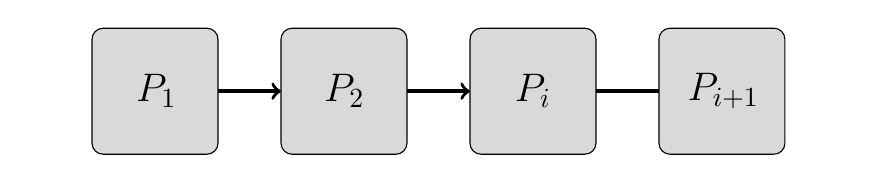
\begin{tikzpicture}[scale=0.8]
\draw[rounded corners, fill=gray!30] (0,0) rectangle (2,2);
\node[align=center, text width=3cm] at (1,1) {\Large $P_1$};

\draw[->, line width=1.25pt] (2,1) -- (3,1);

\draw[rounded corners, fill=gray!30] (3,0) rectangle (5,2);
\node[align=center, text width=3cm] at (4,1) {\Large $P_2$};

\draw[->, line width=1.25pt] (5,1) -- (6,1);

\draw[rounded corners, fill=gray!30] (6,0) rectangle (8,2);
\node[align=center, text width=3cm] at (7,1) {\Large $P_i$};

\draw[->, line width=1.25pt] (8,1) -- (10,1);

\draw[rounded corners, fill=gray!30]  (9,0) rectangle (11,2);
\node[align=center, text width=3cm] at (10,1) {\Large $P_{i + 1}$};
\end{tikzpicture}
\end{center}

The computed facts (the IDB) of $P_i$ become the facts (the EDB) of $P_{i + 1}$.
\begin{itemize}
    \item Critically, we must partition the predicate symbols such that if $p$
    depends on $q$ then $q$ occurs in an earlier or the same program. 
\end{itemize}
\end{frame}

\begin{frame}[fragile]{Example}
The Datalog program: 

\begin{lstlisting}[language=flix, xleftmargin=0.8cm]
Path(x, y) :- Edge(x, y).
Path(x, z) :- Path(x, y), Edge(y, z).
Unconnected(x, y) :- Vertex(x), Vertex(y), not Path(x, y).
\end{lstlisting}

\pause

is stratified as shown by the partition:
%
$$
P_0 = \{ \textsf{Edge}, \textsf{Path}, \textsf{Vertex} \} 
\qquad \text{and} \qquad
P_1 = \{ \textsf{Unconnected} \} 
$$
\end{frame}

\begin{frame}{Precedence Graph}
Given a Datalog program $P$, we define the precedence graph $\mathcal{PG}$:

\begin{itemize}
    \item If there is a rule $A \Leftarrow \cdots, B, \cdots$ then there is an
    edge $A \stackrel{+}\leftarrow B$.
    \item If there is a rule $A \Leftarrow \cdots, \textbf{not} \, B, \cdots$
    then there is an edge $A \stackrel{-}\leftarrow B$.
\end{itemize}

\pause

\textbf{Theorem.} A Datalog program $P$ is stratifiable if and only if its
precedence graph $\mathcal{PG}$ contains no cycle with an edge labeled $-$.
\end{frame}

\begin{frame}[fragile]{Example}
\begin{columns}
\begin{column}{.55\textwidth}
The Datalog program:
\begin{lstlisting}[language=flix]
Husband(x)  :- Man(x), Married(x).
Bachelor(x) :- Man(x), not Husband(x).
\end{lstlisting}

is stratified with the graph on the right.
\end{column}  
\begin{column}{.45\textwidth}
\tikzset{node/.style={circle, fill=black!20, minimum size=4em, align=center, style={font=\scriptsize}}}
\begin{tikzpicture}
    \node [node] at (0,0) (bachelor) {\textbf{Bachelor}};
    \node [node] at (1,2) (husband) {\textbf{Husband}};
    \node [node] at (4,1) (man) {\textbf{Man}};
    \node [node, fill=black!20] at (3,4) (married) {\textbf{Married}};

    \draw[->, thick, red] (man) -- (bachelor) node[midway, above left] {\LARGE -};
    \draw[->, thick] (man) -- (husband) node[midway, above right] {\LARGE +};
    \draw[->, thick] (married) -- (husband) node[midway, above left] {\LARGE +};
    \draw[->, thick] (husband) -- (bachelor) node[midway, above left] {\LARGE +};
\end{tikzpicture}
\end{column}%
\end{columns}
\end{frame}
    
\begin{frame}[fragile]{Example}
\begin{columns}
\begin{column}{.55\textwidth}
The Datalog program:
\begin{lstlisting}[language=flix]
Husband(x)  :- Man(x), not Bachelor(x).
Bachelor(x) :- Man(x), not Husband(x).
\end{lstlisting}

is \emph{not} stratified with the graph on the right.
\end{column}  
\begin{column}{.45\textwidth}
\tikzset{node/.style={circle, fill=black!20, minimum size=4em, align=center, style={font=\scriptsize}}}
\begin{tikzpicture}
    \node [node] at (0,0) (bachelor) {\textbf{Bachelor}};
    \node [node] at (1,2) (husband) {\textbf{Husband}};
    \node [node] at (4,1) (man) {\textbf{Man}};

    \draw[->, thick] (man) -- (bachelor) node[midway, above left] {\LARGE +};
    \draw[->, thick] (man) -- (husband) node[midway, above right] {\LARGE +};
    \draw[->, thick, red] (bachelor) -- (husband) node[midway, above left] {\LARGE -};
    \draw[->, thick, red] (husband) -- (bachelor) node[midway, below right] {\LARGE -};
\end{tikzpicture}
\end{column}%
\end{columns}
\end{frame}

\begin{frame}{Computing the Strata}
We can use the precedence graph $\mathcal{PG}$ to compute the strata:

\begin{enumerate}
    \item Compute the precedence graph $\mathcal{PG}$.
    \item Compute the strongly connected components of $\mathcal{PG}$.
    \item Compute a topological sort of the strongly connected components to
    determine an ordering of the strata.
\end{enumerate}

\medskip

\pause

\centering
\tikzset{node/.style={circle, fill=black!20, minimum size=4em, align=center, style={font=\scriptsize}}}
\begin{tikzpicture}
    \node [node] at (0,0) (married) {\textbf{Married}};
    \node [node] at (3,0) (man) {\textbf{Man}};
    \node [node] at (6,0) (husband) {\textbf{Husband}};
    \node [node] at (9,0) (bachelor) {\textbf{Bachelor}};

    \draw[->, thick] (married) edge[bend left] node[midway, above] {\LARGE +} (husband);
    \draw[->, thick] (man) edge[bend right] node[midway, below] {\LARGE +} (bachelor);
    \draw[->, thick] (man) -- (husband) node[midway, above] {\LARGE +};
    \draw[->, thick, red] (husband) -- (bachelor) node[midway, above] {\LARGE -};
\end{tikzpicture}
\end{frame}

\begin{frame}{Stratified Negation}
We don't actually have to compute the precedence graph or any stratification.
\begin{itemize}
    \item Any half-decent Datalog engine will automatically stratify the program for us.
    \item However, we must understand stratification, to understand when Datalog
    programs with negation are actually meaningful.
\end{itemize}
\end{frame}

\begin{frame}{Summary}
Declarative Programming
\begin{itemize}
    \item the \textbf{\emph{what}}, not the \textbf{\emph{how}}.
\end{itemize}

\pause

Logic programming
\begin{itemize}
    \item programs as logic constraints: \textbf{\emph{facts}} and \textbf{\emph{rules}}.
\end{itemize}

\pause

\textbf{Datalog} is a simple, yet powerful \emph{declarative} \emph{logic}
programming language.
\begin{itemize}
    \item Model-Theoretic Semantics
    \item Fixpoint Semantics
    \item Stratified Negation
\end{itemize}
\end{frame}

\begin{frame}[standout]
\end{frame}

\end{document}
